\chapter{The Set Covering Machine}\label{ch:scm}

First presented by~\cite{marchand02}, the `Set Covering Machine' is an algorithm 
that extends the works of~\cite{valiant} and~\cite{haussler88} to conduct binary
classifications.
These classifications are in an `\texttt{IF \(b_1\) AND \dots AND \(b_n\) THEN class 1 ELSE class 0}'
syntax, using a small logical conjunction or disjunction~\citep{taudien}.
The main goal of the SCM is therefore to find, or at least to approximate, the underlying function that maps data samples to their classes
and thus to minimize the chance of incorrectly classifying an input~\citep{drouin16}.

As the SCM is a supervised machine learning algorithm~\citep{haussler88}, it follows the schema depicted in \autoref{fig:learning_structure}.
It first produces a model, the classification rule, by learning on labeled training samples.
Afterwards the algorithm shall be able to predict the classes of unlabeled test data.
For these predictions, the accuracy, that equals one minus the generalization error, as well as the
sensitivity, i.e.\ the fraction of correctly classified class 1 samples, and the specificity,
i.e.\ the fraction of correctly classified class 0 samples, can be characterized.

\begin{figure}[ht]
    \centering
    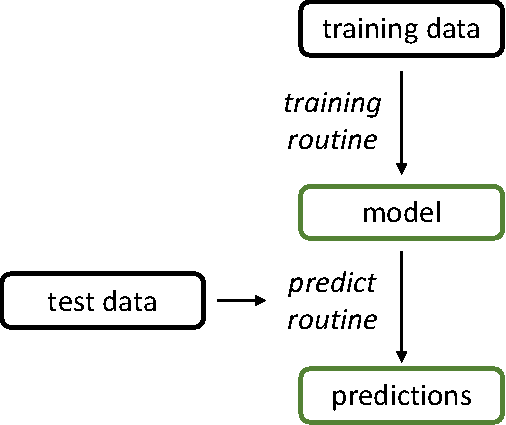
\includegraphics[width=0.55\columnwidth]{figures/learning_structure.pdf}
    \caption{General structure of a supervised learning algorithm. Inspired by~\cite{valiant}.}\label{fig:learning_structure}
\end{figure}

In the following sections, the algorithm, the underlying greedy set cover (see \autoref{sec:setCover}) and the SCM's predecessors (see \autoref{sec:origin}) are outlined.
First, original SCM for classifying data with a binary set of features (\autoref{sec:basicSCM}) is described, followed by short
introductions to different base classifiers like data-dependent balls (\autoref{subsec:balls}) and rays (\autoref{subsec:rays}).

%%%%%%%%%%%%%%%%%%%%%%%%%%%%%%%%%%%%%%%%%%%%%%%%%%%%%%%%%%%%%%%%%%%%%%%%%%%%%%%%%%%%%%%%%%%%
\section{Motivation and Requirements to the SCM}

% why no SVM?
While it seems like a good choice to just use the well-established support vector machine (SVM) by~\cite{cortes} for classification tasks, that might not always be the case.
The SVM algorithm constructs hyperplanes, along which it separates the two classes of data~\citep{cristianini}.
However this use of mainly linear hyperplanes for classification, makes the resulting models
quite complex, stiff and unintuitive to interpret for humans~\citep{marchand02}.

% produce sparse classifiers
The aim of the SCM is instead to produce a very simple, sparse and thus easy to interpret classifier that
clearly demonstrates the importance of each feature~\citep{drouin16}.
Linear separability of the data shall not be a requirement for the classification algorithm to work correctly~\cite{marchand02}.
Conjunctions are perfect for this task, as they are especially easy to understand for humans.
Having a simple rule as the algorithm's result, is furthermore beneficial, as it makes the SCM extremely valuable for scientific purposes,
as those rules are comparatively easily validatable using literature or even lab-experience~\citep{drouin16}.
They might also expose or verify hypotheses, or even set off future research by providing new insights~\citep{kestler11}.

% balance between short and accurate needed
It is the overall goal of every supervised learning algorithm to obtain classifiers with low generalization errors,
i.e.\ a good performance on unknown, independent test data.
To achieve such a low generalization error, both, the sparseness and the training accuracy of the decision rule, should be be maximized~\citep{marchand02}.
Yet, since the accuracy and the sparsity of a classifier are usually opposing goals~\citep{drouin16},
this is no easy problem and requires some elaborate balancing.
On the one hand side an extremely compact decision rule might only incorporate very few features and thus provide no feasible result at all.
On the other hand side, a very accurate classification rule might classify all test samples correctly, but come along with low interpretability and a
very high generalization error when applying the classifier to the test data.

% many features and few samples
Moreover, since the SCM is supposed to be a general-purpose learning machine,
the algorithm is in general able to deliver feasible results, even when confronted with a data set of a
very high feature dimension and low sample cardinality~\citep{kestler11}.
As data sets with tens of thousands of features and only a few hundred samples are not uncommon
in real-world problems and especially in biomedical learning tasks~\citep{lausser20}.
Yet the SCM is only expected to deliver good results, when very few features are actually informative.
This, however, is a minor requirement, since it is usually the case in real-world data sets.
The aim of the SCM is hence to bring order to this huge chaos of relevant and irrelevant features,
by picking only the few most relevant ones and forming them into a sparse logical conjunction, or disjunction, that is ordered by the features relevance,
as the most important feature is supposed to be added to the decision rule first~\citep{marchand02}.

%%%%%%%%%%%%%%%%%%%%%%%%%%%%%%%%%%%%%%%%%%%%%%%%%%%%%%%%%%%%%%%%%%%%%%%%%%%%%%%%%%%%%%%%%%%%
\section{Definitions}\label{sec:definitions}

% input space, classification rule
As its input, the basic SCM receives a binary data set \(S \in \lbrace0,1\rbrace^{m \times n}\) with
\(n\) attributes as its columns and \(m\) samples \(x \in \lbrace0,1\rbrace^{n}\) as its rows~\citep{marchand02}.
Additionally each sample has a label \(y \in \lbrace0,1\rbrace\).
Even though, as~\cite{schmid} showed, unlabeled samples could technically be incorporated into the training algorithm by using specific procedures,
this mechanism is not used in this thesis.
The goal of the SCM is now to find a good decision rule, also called `classifier' or `classification rule',
\(f: X \rightarrow Y = \lbrace0,1\rbrace\) that maps any sample of the input space \(X\) to its corresponding label \(y \in Y = \lbrace0,1\rbrace\).
% classification rule = set of multiple classifiers?!
The sample's classes, namely usually `class 0' and `class 1', will also be referred to as the `negative' and `positive' samples.

% attributes vs features
~\cite{marchand02} furthermore differentiate between `attributes' and `features'.
While attributes are usually Boolean valued, features can be of a more complex form.
Besides Boolean features, there are various other kinds of features such as rays (\autoref{subsec:rays}) and balls (\autoref{subsec:balls}).
Those more complex types of features are usually data-dependent, meaning that they were constructed from the available training data.
But in the end, all these features are essentially characteristics --- like `\texttt{\(x_5\) = true}' in case of Boolean features --- a sample either does or does not have.
Thus features are defined by~\cite{marchand02} as functions that evaluate to true or false given any sample \(x \in X\).

% base classifiers
On the other hand, `base classifiers' \(b_i\) are the first level (also known as `base' level) building blocks of the resulting classification rule~\citep{kestler11}.
`\texttt{\(x_9 < 7\)}' could for example be one of them, in case rays are used as base classifiers. % otherwise: base classifier = feature type

%%%%%%%%%%%%%%%%%%%%%%%%%%%%%%%%%%%%%%%%%%%%%%%%%%%%%%%%%%%%%%%%%%%%%%%%%%%%%%%%%%%%%%%%%%%%
\section{The Greedy Set Cover}\label{sec:setCover}

The minimum set cover problem on the data set \(S \in \lbrace0,1\rbrace^{m \times n}\) of m samples and n attributes is defined as follows.
It tries to cover each of the samples by at least one of the available attributes, each covering 0 to m of those elements.
A column j `covers' an element i, if and only if \(s_{ij} = 1\).
Additionally there usually is a cost vector \(c \in \mathbb{R}_{+}^{n} \) that associates a cost value to every column.
In the context of the SCM, the cost of every attribute is however set to one.
The goal of the set cover problem is now to find a subset of attributes that is of minimal cost and covers all m samples at least once~\citep{caprara}.

There are multiple ways of finding such a minimum set cover, that can be assigned mainly into the classes of exact, linear and heuristic algorithms~\citep{caprara}.
As the set cover problem is NP-complete, exact algorithms are barely realizable in the context of big data sets, because of their high worst case execution time bounds~\citep{chvatal}.
However, there exists an easy approach using a greedy heuristic, that has only polynomial worst case execution time introduced by~\cite{chvatal}.
A greedy algorithm in general solves an optimization problem by using the simple principle, 
of always choosing the current optimum for iteratively extending the solution.
This technique usually involves a loss of outcome optimality, hence the solution is usually only an approximation of the optimum,
yet, the algorithm benefits from a very fast computation time and often still results in feasible results~\citep{cormen}.

\begin{algorithm}[ht]
    \KwIn{S}
    uncovered samples = every line of S\\
    cover = \(\emptyset\)
    \While{uncovered samples \(\neq \emptyset\)}{
        Select attr \(\in\) S that covers the highest number of uncovered samples.\\
        uncovered samples = uncovered samples - attr \\
        cover = cover \(\cup\) \{attr\}
    }
    Return cover.
    \caption{The greedy set cover algorithm, as described by~\cite{chvatal}.}\label{code:greedySetCover}
\end{algorithm}

The `greedy set cover' algorithm, illustrated in \autoref{code:greedySetCover}, thus recursively selects the optimal sets.
After each iteration, it deletes the covered samples from the list of remaining ones.
Once all samples are covered, the algorithm stops and the subset of all selected sets is returned as the solution.
This greedy approach actually delivers a feasible minimum set cover with a proven, tight worst case bound that guarantees the
cost of the resulting greedy cover to be less than or equal \(H(d) \times \) the cost of the optimal cover~\citep{chvatal}.
Here \( H(d) = \sum_{i=1}^d \sfrac{1}{i} \) denotes the harmonic numbers with the size \(d\) of the largest set as its parameter.

%%%%%%%%%%%%%%%%%%%%%%%%%%%%%%%%%%%%%%%%%%%%%%%%%%%%%%%%%%%%%%%%%%%%%%%%%%%%%%%%%%%%%%%%%%%%
\section{The SCM's Predecessors}\label{sec:origin}

The SCM has its earliest origins in the algorithm of~\cite{valiant} for PAC learning a conjunctive binary classifier of Boolean attributes.
This approach was later optimized by~\cite{haussler88}, who reduced the classifier's complexity by applying the greedy set cover.

The following section gives a summary of the advancements and problems of early conjunction and disjunction learning algorithms.
All the algorithms in this section are applicable to both, conjunctions and disjunctions.
The disjunctive case can simply be obtained by switching the roles of the positive and negative training samples and applying trivial logical equivalences.

%%%%%%%%%%%%%%%%%%%%%%%%%%%%%%%%%%%%%%%%%%%%%%%%%%%%%%%%%%%%%%%%%%%%%%%%%%%%%%%%%%%%%%%%%%%%
\subsection{Valiant's Algorithm for Learning Conjunctions}

In his paper `A Theory of the Learnable'~\cite{valiant} introduced the concept of probably approximately correct (PAC) learnability.
He categorizes certain classes of binary classification problems as PAC learnable and constructs a two-step machine for PAC learning these problems in a supervised manner
with the goal of approximating their underlying classification functions at a high probability.
In this algorithm the teacher first gives the learner access to training samples using a specific learning protocol.
Here the learner can request randomly chosen positive samples or get the classification of an own sample to verify its tendencies.
In the following deduction procedure the learner now uses its knowledge from the learning first phase to derive a concept in the form of a Boolean function/expression.

Even though the resulting PAC classifier is not guaranteed to be correct, it is guaranteed to have a sensitivity of 100\% and a specificity \(< \varepsilon \)
forcing the probability of a false negative to be adjustable low, provided there are enough training samples available to the learner (precise bounds can be found in~\cite{valiant}).
This deduction procedure runs in polynomial time and thus forms a wide-spread base framework for developing efficient and probably correct learning algorithms~\citep{haussler90}.

~\cite{valiant} subsequently applies this PAC approach to constructing an algorithm to learn a conjunction or disjunction of Boolean attributes.
This algorithm uses the training samples to find a \(C \subseteq H\) containing exactly those attributes of the attribute set \(H\)
that correctly classify all of the positive training samples~\citep{marchand02}.
The conjunction of any \(c \in C\) is therefore also correctly classifies all positive training samples, giving each conjunction a sensitivity of 100\%.
To now also achieve the best possible results on the negative training samples, the conjunction of all \(c \in C\)  is formed and returned
as the chance of classifying a sample, that's not included in the set of positive samples, as negative
and therefore increasing the rules specificity, rises with every term that is added to the conjunction.
Yet this final decision rule is not guaranteed to be consistent with all of the negative samples or any of the unknown test samples.

However the requirement for a attribute to be consistent with all positive samples leads to an overfitting of the classifier
and wastes potential by not taking the negative samples into account~\citep{haussler88,marchand02}.
Additionally, the resulting conjunction may depend on a great number of attributes.
This high complexity most often leads to a decreased interpretability of the classifier,
as well as a high generalization error on unknown test samples.

%%%%%%%%%%%%%%%%%%%%%%%%%%%%%%%%%%%%%%%%%%%%%%%%%%%%%%%%%%%%%%%%%%%%%%%%%%%%%%%%%%%%%%%%%%%%
\subsection{Haussler's Two-Step Algorithm for Learning Sparse Conjunctions}

~\cite{haussler88} recognized the increased generalizability of compact classifiers and thus extended Valiant's algorithm accordingly.
In a two-step algorithm he first executes Valiant's algorithm to PAC learn a set \(C\) of Boolean attributes
that are all consistent with every sample.
As the second step he then uses the greedy set cover, with its tight bounds regarding the results accuracy and the execution time,
to reduce this attribute set to its smallest possible subset \(R \subseteq C\).
The conjunction of the subset's attributes has to correctly classifies all negative training samples, in order for \(R\) to be a valid solution.
If such a set does not exist, which happens quite often when working with complex real-world data, it returns no solution at all.
Yet whenever there actually exists set of attributes that is consistent with all training samples, 
Haussler's algorithm is guaranteed to find such a set as the solution~\citep{marchand02}.
Even more, this greedily obtained solution will be found in a time that is only polynomial in terms of \(n\) and \(m\)~\citep{kestler06}.
The classifier itself is bounded to be only by a factor of \(\ln m\) bigger than the optimal set of attributes \(s\)~\citep{marchand04,kestler06}.

Moreover this means, that the classifier's size does not depend on the total number of attributes \(n\), but only on the
number of relevant attributes \(s\), allowing the algorithm to perform well even if \(m << n\), as long as \(s \approx m\)~\citep{kestler06}.
In the end, the algorithm Haussler's algorithm returns a conjunction as the decision rule that is far more compact
than the original conjunction of Valiant and therefore has a way higher chance of a good generalizability.

But after all, the algorithms of~\cite{valiant} and~\cite{haussler88} have two major downsides:
Firstly they only work with Boolean attributes and secondly there is no possibility to adjust the level of the tradeoff
between the classifier's accuracy in training and its complexity~\citep{marchand02}.
Yet, this tradeoff is badly needed, as real-world data usually contains a lot of noise that can only be
filtered out by reducing the conjunctions accuracy and therefore improving the models ability to generalize~\citep{marchand02}.
To address these problems~\cite{marchand02} created the `set covering machine' algorithm.

%%%%%%%%%%%%%%%%%%%%%%%%%%%%%%%%%%%%%%%%%%%%%%%%%%%%%%%%%%%%%%%%%%%%%%%%%%%%%%%%%%%%%%%%%%%%
\section{The Basic Set Covering Machine}\label{sec:basicSCM}

~\cite{marchand02} generalized and extended Haussler's two-step algorithm by introducing the model selection hyper-parameters \(p\) and \(s\).
The penalty for misclassifying a positive sample \(p\) allows the users to control the trade-off between making errors on positive versus on negative samples.
On the other hand the early stopping point \(s\) lets them trade-off between an accurate classifier,
that is consistent with as many samples as possible, and a sparse classifier, that is easy to interpret and more generalized.
Additionally he replaced the Boolean attributes by Boolean valued features (see \autoref{sec:definitions}) that may be more complex, than ordinary attributes. 

The precise adjusting of the hyperparameter \(p\) comes in very handy, as both, conjunctions and disjunctions, have heavily asymmetrical behaviors.
A sample will only be classified as positive by a conjunction, if it is consistent with all base classifiers.
However, inside a disjunction, a sample will be classified as positive, once it is consistent with even just a single base classifier~\cite{schmid}.
In the case of a conjunction \(p\) should therefore usually prioritize the correctness of positive samples by being \(> 1\),
thus leading to an increased sensitivity of the the base classifier.
In the case of a disjunction the opposite should occur.
In addition \(p\) can also be used for balancing the classifiers sensitivity and specificity
depending on the ratio of positive training samples to negative training samples.
In the corner case of \(p = \infty\), a features has to be consistent with all positive samples in order to be selected,
like in Haussler's original algorithm~\citep{kestler06}.

The BuildSCM algorithm (\autoref{code:buildSCM}) has a worst case runtime complexity of only \(\mathcal{O} (m \cdot |H| \cdot s)\)~\citep{drouin16},
making it high performant even on large data sets.
When building a conjunction, a sample is removed from all remaining sets within the algorithm and requires no further consideration,
once it is classified as negative by a selected feature \(h_k \in Res\), as it has no chance to be reclassified anymore.
The same happens to samples that get classified as positive when constructing a disjunction.

The expression `\(|Q_i| - p \cdot |R_k|\)' quantifies a feature's usefulness~\citep{marchand02}.
This score however changes dynamically whenever a new, especially useful, feature is picked greedily as the next base classifier in every iteration,
as the feature's sets \(Q\) and \(R\) get effected directly.
The selection of a feature therefore always depends on the selection of the previously chosen features.
Yet, the selected feature \(h_k \in H\) may remain in \(H\),
as both \(Q_k\) and \(R_k\) are now empty sets anyhow, meaning that \(h_k\) will never again
have a usefulness score other than zero and thus will never be considered for \(Res\) anymore.
Once every negative sample \(n \in N\) is covered or \(s\) iterations have been executed
the resulting classification rule, here a simple conjunction or disjunction of Boolean features, is returned.

\begin{algorithm}[ht]
    \KwIn{
        \\ \(S\) --- training data set
        \\ \(p\) --- penalty value for a misclassification
        \\ \(s\) --- maximum amount of base classifiers that may be used in the rule
        \\ \(H\) --- set of Boolean valued features \(h_i(x)\)}
    \KwOut{sparse conjunction/ disjunction of \(Res \subseteq H\)}
    \(Res = \emptyset\) \\
    \(P =
    \begin{cases}
        \text{set of positive training samples,} & \text{conjunctive SCM} \\
        \text{set of negative training samples,} & \text{disjunctive SCM}
    \end{cases}\) \\
    \(N =
    \begin{cases}
        \text{set of negative training samples,} & \text{conjunctive SCM} \\
        \text{set of positive training samples,} & \text{disjunctive SCM}
    \end{cases}\) \\
    \For{\(h_i \in H\)}{
        \(Q_i\) = subset of \(N\)'s elements that are consistent with the assumption of \(h_i\) \\
        \(R_i\) = subset of \(P\)'s elements that are inconsistent with the assumption of \(h_i\)
    }
    \While{\(|N| > 0\) and \(|Res| < s\)}{
        \(h_k\) = feature \(h_i \in H\) with the maximum value of \(|Q_i| - p \cdot |R_k|\) \\
        \(Res = Res \cup \{h_k\}\) \\
        \(N = N - Q_k\) \\
        \(P = P - R_k\) \\
        \For{\(h_i \in H\)}{
            \(Q_i = Q_i - Q_k\) \\
            \(R_i = R_i - R_k\)
        }
    }
    Return \(f(x) =
    \begin{cases}
        \bigwedge_{i \in Res} h_i(x), & \text{conjunctive SCM} \\
        \bigvee_{i \in Res} h_i(x), & \text{disjunctive SCM}
    \end{cases}\)
    \caption{The basic `BuildSCM' algorithm for Boolean features. Created according to~\cite{marchand02}.}\label{code:buildSCM}
\end{algorithm}

The SCM always only approximates the optimal solution, as it is using a greedy algorithm.
Nevertheless~\cite{marchand02} observed, that if there actually exists a sparse conjunction or disjunction with few errors on the training data,
the correctly adjusted BuildSCM algorithm will most likely identify this classifier.
This further implies that the algorithm performs well, even when working on a data set with far more features than samples,
provided that only few of those features are actually relevant for a classification.
Overall the SCM benefits highly from its simplicity, both of the algorithm itself and the resulting classifiers,
and the high compression rate that is achieved by compression the main information of a huge data set into
just a small rule, that can even be stores as a simple string.

%%%%%%%%%%%%%%%%%%%%%%%%%%%%%%%%%%%%%%%%%%%%%%%%%%%%%%%%%%%%%%%%%%%%%%%%%%%%%%%%%%%%%%%%%%%%
\section{Extending the SCM by Different Base Classifiers}\label{sec:baseClassifiers}

Besides this SCM for Boolean features with classification rules like `\texttt{IF x1 AND x4 THEN class 1}',
there are many different types of base classifiers that can be employed for the decision rules~\citep{kestler11}.
The data set is now in general defined as \(S \in \mathbb{R}^{m \times n}\), instead of only \(S \in \lbrace0,1\rbrace^{m \times n}\).
This makes the SCM easily applicable to a whole new group of real-world data sets, like gene expression data.
Good base classifiers shall have good compression rates,
meaning that they reduce the dimension of the data set by a lot by encoding the information into a more compact notation.
This compression rate is usually measured as the ratio of the SCM's input, the sample set, to its output, the classifier.
It assumes that the algorithms output contains all important sample information.

Since data-dependent balls and data-dependent rays can be considered as the two most promising and widespread base classifiers,
their concepts are introduced in the following.
But there are many more noteworthy types of base classifiers like data-dependent half spaces 
that~\cite{marchand03} developed as an extension to the concept of data-dependent balls.

%%%%%%%%%%%%%%%%%%%%%%%%%%%%%%%%%%%%%%%%%%%%%%%%%%%%%%%%%%%%%%%%%%%%%%%%%%%%%%%%%%%%%%%%%%%%
\subsection{Using Data-Dependent Balls as Features}\label{subsec:balls}

~\cite{marchand02} first introduced the concept of having a set of spheres, that are centered around training samples, as the set of features.
The SCM here successively selects the most favorable balls, according to a specific heuristic, for the resulting conjunction or disjunction~\citep{germain}.
Using the PAC framework,~\cite{marchand02} give a tight bound for the generalization error of this SCM
in terms of the achieved amount of sample compression.

Each feature
\[h_{i,p}(x) \mathrel{\mathop:}= h_p(x,x_i) =
\begin{cases}
    y_i, & d(x,x_i) \leq p \\
    \overline{y_i}, & else
\end{cases}\]
is defined as the inside of a sphere around one training sample \(x_i\) with the radius \(p \in \mathbb{R}\) and
the distance \(d(x,x_i)\) between the points \(x\) and \(y\), that may be calculated using any common distance metric~\citep{marchand02}.
A sample is therefore classified using its proximity to other samples~\citep{germain}.
This however leads to a very complex model, as the distances of every feature to every other feature need to be computed and stored,
making the runtime complexity of this SCM with data-dependent balls exponential in the number of samples and therefore very high.

%%%%%%%%%%%%%%%%%%%%%%%%%%%%%%%%%%%%%%%%%%%%%%%%%%%%%%%%%%%%%%%%%%%%%%%%%%%%%%%%%%%%%%%%%%%%
\subsection{Using Data-Dependent Rays as Features}\label{subsec:rays}

Shortly after the concept of building an SCM that uses data-dependent rays as its set of features was first introduced by~\cite{marchand04},
~\cite{kestler06} picked it up, extended it and used for microarray analyses.
The application of this SCM type on gene expression data, or in general many types of real-world data with real-valued features, works very well and
provides valuable information on the underlying patterns by its simple and easily to interpret classification classification rules~\citep{marchand04,kestler06,kestler11}.
Moreover it works well on data of high feature dimension and low cardinality, in which case there is a high
chance of one ray being perfectly consistent with all samples.
I will therefore use these data-dependent rays for the following analysis of high-dimensional RNA-seq data.

A `single threshold classifier' (STC) is defined as a classifier, that predicts the label of a sample,
according to a single threshold \(t\), that only depends on a single feature \(h_i \in \mathbb{R}\) of the sample \(x_j\)~\citep{kestler11,marchand04}.
`x5 = 4.1' could for example be such a STC.\
Rays use these STCs and expand them by a direction to produce rules in the form of `\(\text{feature}_x \geq \text{threshold}_y\)' and `\(\text{feature}_x < \text{threshold}_y\)'~\citep{marchand04}.
This direction can for example be be defined binary as \(d \in \{-1,1\}\), allowing the definition of a ray as
\[r(x) =
\begin{cases}
    1, & (x_{ij} - t)d \geq 0 \\
    0, & else
\end{cases}\]~\citep{kestler11}.
According to~\cite{kestler11}, a ray is called `data-dependent', if its threshold is placed directly on top of a data sample.
In general the features are not input separately into the algorithm in form of a feature set \(H\), but are directly derived from the data set \(S\),
when using data-dependent rays.

% interval vs rays
As rays are basically half-open intervals~\citep{kestler11}, the conjunction of an ensemble of rays forms a, usually partially open, hyper-rectangle in the input space,
with the ray's thresholds being the hyper-rectangle's borders.
The SCM with rays as base classifiers is in general very high performant, even in the context of high-dimensional data sets~\citep{kestler11}.
~\cite{kestler06} bounded the generalization error of the SCM with data-dependent rays as its set of features based on the Vapnik-Chervonenkis (VC) dimension of the base classifier space.
Those bounds were then tightened by new error bounds, this time based on the amount of data compression this version of the SCM achieves on its training data.
~\cite{kestler11} furthermore constructs and proves a good sample compression bound for this version of the SCM.\